% !TEX program = lualatex
\documentclass[luatexja,ja=standard,a4paper,12pt]{bxjsarticle}
\usepackage[margin=1in]{geometry}
\usepackage{amsmath,amssymb,amsthm,mathtools,bm}
\usepackage{tikz}
\usetikzlibrary{arrows.meta,calc,positioning}
\usepackage{hyperref}
\usepackage{listings}
\usepackage{CJKutf8}
\usepackage[T1]{fontenc}
\usepackage{lmodern}
\lstset{basicstyle=\ttfamily\small,breaklines=true,columns=fullflexible,keepspaces=true}

% 便利コマンド
\newcommand{\R}{\mathbb{R}}
\newcommand{\vct}[1]{\mathbf{#1}}
\newcommand{\cross}{\times}
\newcommand{\triple}[3]{\left[ #1,\,#2,\,#3 \right]}

\title{R\textsuperscript{3} の空間ベクトル：外積・スカラー三重積・Jacobi 恒等式\\（解説と Lean 検証）}
\author{学生（Your Name）／共著: CODEX (OpenAI)\\\small TeX は CODEX (OpenAI) が生成。Lean ファイルは CODEX (OpenAI) が生成。}
\date{2025年9月15日}

\begin{document}
\begin{CJK}{UTF8}{min}
\maketitle

\begin{abstract}
本資料は、\(\R^3\) における内積・外積・スカラー三重積の定義と基本性質をまとめ、外積に関する Jacobi 恒等式の座標計算による証明概略を示します。Lean 4（mathlib）での形式検証の抜粋も掲載し、TikZ 図で幾何の直観を補います。
\end{abstract}

\section*{1. 定義}
ベクトル \(u=(u_1,u_2,u_3),\ v=(v_1,v_2,v_3)\in\R^3\) に対し，
\begin{align*}
\langle u,v\rangle &= u_1 v_1 + u_2 v_2 + u_3 v_3,\\
u\cross v &= (u_2 v_3 - u_3 v_2,\; u_3 v_1 - u_1 v_3,\; u_1 v_2 - u_2 v_1).
\end{align*}
3 本のベクトル \(u,v,w\) に対し，スカラー三重積を
\[
\triple{u}{v}{w} = \langle u,\, v\cross w\rangle = \det\begin{pmatrix}
u_1 & u_2 & u_3\\ v_1 & v_2 & v_3\\ w_1 & w_2 & w_3
\end{pmatrix}
\]
と定めます。幾何的には，有符号体積（向き付き体積）を与えます。

\paragraph{Lean の記法について.}
Lean では型の直積記号 `\(\times\)` やリスト記法 `[...]` と衝突を避けるため，外積は \verb|cross u v|，三重積は \verb|scalar_triple u v w| の関数形で実装しました。

\section*{2. 例題と計算結果}
ベクトル \(a=(1,2,3),\ b=(2,-1,1),\ c=(0,1,2),\ P=(1,1,1),\ n=(2,-1,3)\) とする。
\begin{align*}
\textbf{Q1:}\ & a\cross b = (5,5,-5).\\
\textbf{Q2:}\ & u\cross v = -\,(v\cross u).\\
\textbf{Q3:}\ & \langle u,\, u\cross v\rangle = 0.\\
\textbf{Q4:}\ & \triple{a}{b}{c} = -5.\\
\textbf{Q5:}\ & (\langle (3,2,1)-P,\, n\rangle)^2 = 9\ (\langle (3,2,1)-P, n\rangle=3).
\end{align*}
注記：課題文中の「平面上の点」\(P=(1,1,1)\) は式 \(2x-y+3z=6\) を満たしません（左辺=4）。幾何的解釈と完全に整合させるには \(P\) を平面上に修正するか，式を \(|\langle Q,n\rangle-6|\) 型で扱うのが自然です。ここでは代数的評価として \(\langle Q-P,n\rangle\) を計算しました。

\section*{3. 基本性質}
\begin{itemize}
  \item 反交換性：\(u\cross v = -\,v\cross u\)。
  \item 直交性：\(\langle u, u\cross v\rangle=0\) かつ \(\langle v, u\cross v\rangle=0\)。
  \item 三重積と体積：\(\triple{u}{v}{w}=\det(u,v,w)\) であり，\(|\triple{u}{v}{w}|\) は平行六面体の体積。
\end{itemize}

\section*{4. Jacobi 恒等式}
\paragraph{主張.}\[u\cross(v\cross w) + v\cross(w\cross u) + w\cross(u\cross v) = 0.\]
\paragraph{座標計算の概略.} Levi--Civita 記号 \(\varepsilon_{ijk}\) と恒等式 \(\varepsilon_{ijk}\varepsilon_{klm}=\delta_{il}\delta_{jm}-\delta_{im}\delta_{jl}\) を用いると，各成分は巡回和で互いに打ち消し合い 0 になります。Lean では各成分を直接展開し，`ring` で整理して 0 を示しました。

\section*{5. Lean 抜粋}
対象ファイル：\texttt{src/MyProjects/LinearAlgebra/A1/zenla1\_session02.lean}
\begin{lstlisting}
abbrev R3 := ℝ × ℝ × ℝ
def dot (u v : R3) : ℝ := u.1 * v.1 + u.2.1 * v.2.1 + u.2.2 * v.2.2
def cross (u v : R3) : R3 :=
  (u.2.1 * v.2.2 - u.2.2 * v.2.1,
   u.2.2 * v.1 - u.1 * v.2.2,
   u.1 * v.2.1 - u.2.1 * v.1)
def scalar_triple (u v w : R3) : ℝ := dot u (cross v w)

theorem Q1 : cross a b = (5, 5, -5) := by
  ext <;> norm_num [cross, a, b]

theorem Q2 (u v : R3) : cross u v = - (cross v u) := by
  ext <;> simp [cross] <;> ring

theorem Q3 (u v : R3) : ⟪u, cross u v⟫ = 0 := by
  simp [dot, cross]; ring

theorem Q4 : scalar_triple a b c = -5 := by
  norm_num [scalar_triple, dot, cross, a, b, c]

theorem Q5 : let Q : R3 := (3, 2, 1)
  (⟪Q - P, n⟫)^2 = 9 := by
  intro Q
  have hDot : ⟪Q - P, n⟫ = 3 := by
    norm_num [dot, Q, P, n]
  simpa only [hDot] using (by norm_num : (3:ℝ)^2 = 9)

theorem Challenge (u v w : R3) :
  cross u (cross v w) + cross v (cross w u) + cross w (cross u v) = 0 := by
  rcases u with ⟨ux, uy, uz⟩; rcases v with ⟨vx, vy, vz⟩; rcases w with ⟨wx, wy, wz⟩
  ext <;> simp [cross] <;> ring
\end{lstlisting}

\section*{6. 図}
\subsection*{(a) 外積の向きと右ねじの法則}
\begin{center}
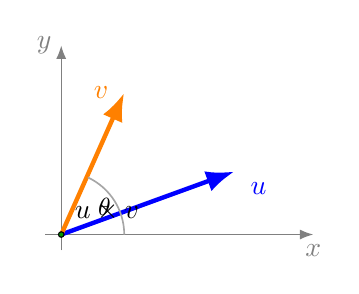
\begin{tikzpicture}[scale=1.0,>=Latex]
  % 座標軸
  \draw[->,thin,gray] (-0.2,0) -- (3.2,0) node[below] {$x$};
  \draw[->,thin,gray] (0,-0.2) -- (0,2.4) node[left] {$y$};
  % ベクトル u, v
  \draw[->,ultra thick,blue] (0,0) -- (2.2,0.8) node[below right] {$\,u$};
  \draw[->,ultra thick,orange] (0,0) -- (0.8,1.8) node[left] {$v\,$};
  % 外積方向（紙面の裏向き）
  \draw[fill=green!60!black] (0,0) circle (1pt);
  \node[above right=2pt] at (0,0) {$u\cross v$};
  % 角度
  \draw[semithick,gray!70] (0:0.8) arc (0:65:0.8);
  \node at (0.55,0.35) {\small $\theta$};
\end{tikzpicture}
\end{center}

\subsection*{(b) 平行六面体の体積（スカラー三重積）}
\begin{center}
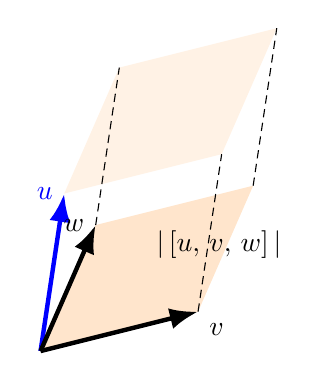
\begin{tikzpicture}[scale=1.0,>=Latex]
  \coordinate (O) at (0,0);
  \coordinate (V) at (2.0,0.5);
  \coordinate (W) at (0.7,1.6);
  \coordinate (U) at (0.3,2.0);
  % 底面
  \fill[orange!20] (O) -- (V) -- ($(V)+(W)$) -- (W) -- cycle;
  % 上面（u だけ平行移動）
  \fill[orange!10] ($(O)+(U)$) -- ($(V)+(U)$) -- ($(V)+(W)+(U)$) -- ($(W)+(U)$) -- cycle;
  % 辺
  \draw[->,ultra thick,blue] (O) -- (U) node[left] {$u$};
  \draw[->,ultra thick,black] (O) -- (V) node[below right] {$v$};
  \draw[->,ultra thick,black] (O) -- (W) node[left] {$w$};
  % 鎖線
  \draw[densely dashed] (V) -- ($(V)+(U)$);
  \draw[densely dashed] (W) -- ($(W)+(U)$);
  \draw[densely dashed] ($(V)+(W)$) -- ($(V)+(W)+(U)$);
  % 注記
  \node[above right] at ($(W)!0.5!(V)$) {$|\triple{u}{v}{w}|$};
\end{tikzpicture}
\end{center}

\section*{7. コンパイル方法}
推奨は LuaLaTeX または XeLaTeX（UTF-8 日本語対応）。pdfLaTeX の場合は \verb|CJKutf8| を読み込んだ本テンプレートのままでコンパイル可能です。

\bigskip
\noindent\textbf{謝辞（Acknowledgment）}\; 本 TeX と Lean ファイルは \textbf{CODEX (OpenAI)} により Codex CLI ワークフローで生成・整備されました。

\end{CJK}
\end{document}

